%-------------------------------------------------------------------------------
%  EEG-Based Directional Brainwave Classification for Assistive BCI Systems
%
%  Final Project Report  -  CS-GY 6513 Big Data  -  NYU Tandon  -  Spring 2026
%
%  Compile with: pdflatex -> bibtex -> pdflatex x2  (no .bib used; refs inline)
%-------------------------------------------------------------------------------
\documentclass[conference]{IEEEtran}
\IEEEoverridecommandlockouts

\usepackage{cite}
\usepackage{amsmath,amssymb,amsfonts}
\usepackage{algorithmic}
\usepackage{graphicx}
\usepackage{textcomp}
\usepackage{xcolor}
\usepackage{booktabs}
\usepackage{multirow}
\usepackage{listings}
\usepackage{url}
\usepackage{hyperref}

% ---- Listings setup (per user pref: lstlisting for pseudocode) ----------------
\definecolor{codegray}{rgb}{0.95,0.95,0.95}
\definecolor{codekey}{rgb}{0.10,0.30,0.65}
\definecolor{codecmt}{rgb}{0.35,0.55,0.35}
\lstset{
  backgroundcolor=\color{codegray},
  basicstyle=\ttfamily\footnotesize,
  keywordstyle=\color{codekey}\bfseries,
  commentstyle=\color{codecmt}\itshape,
  breaklines=true,
  columns=fullflexible,
  showstringspaces=false,
  frame=single,
  framerule=0pt,
  xleftmargin=4pt,
  xrightmargin=4pt,
  aboveskip=6pt,
  belowskip=6pt
}

\hypersetup{
  colorlinks=true,
  linkcolor=black,
  citecolor=black,
  urlcolor=blue!60!black
}

\def\BibTeX{{\rm B\kern-.05em{\sc i\kern-.025em b}\kern-.08em
    T\kern-.1667em\lower.7ex\hbox{E}\kern-.125emX}}

\begin{document}

%==============================================================================
\title{EEG-Based Directional Brainwave Classification
for Assistive BCI Systems}

\author{
\IEEEauthorblockN{Janardhana Reddy MS}
\IEEEauthorblockA{Net ID: jr6922}
\and
\IEEEauthorblockN{Divyansh Maurya}
\IEEEauthorblockA{Net ID: dm6022}
\and
\IEEEauthorblockN{Chiranjeev Kumar}
\IEEEauthorblockA{Net ID: ck4137}
}

\maketitle

%==============================================================================
\begin{abstract}
We present an end-to-end distributed Brain-Computer
Interface (BCI) system that decodes three-class motor-imagery intentions
(left hand, right hand, rest) from streaming electroencephalographic (EEG)
signals. The pipeline combines a two-stage preprocessing chain (ICA cleaning
followed by Spark-based epoch extraction into Delta Lake), a polyglot storage
layer spanning MongoDB, Cassandra, Redis, and pgvector, and a transfer-learning
chain using PhysioNet EEGMMIDB, Cho~2017, and BCI Competition IV-2a data. A
FastAPI inference layer is driven by a Kafka producer and a LangGraph agentic
consumer that performs signal-quality scoring, prediction, session monitoring,
data curation, retrieval, and alerting on each epoch. With 50-shot per-class
calibration, the personalized ensemble reaches 88.1\,\% accuracy on the best
BCI IV-2a subject and 66.5\,\% mean accuracy across all nine subjects, compared
with a 49.6\,\% mean LOSO EEGNet baseline and a 54.4\,\% mean zero-shot
ensemble. We also document one negative result: at the 5-channel scale used by
our deployed pipeline, EEG Conformer underperformed the convolutional baselines
and was deprioritized.
\end{abstract}

\begin{IEEEkeywords}
Brain-Computer Interface, EEG, Motor Imagery, Transfer Learning, Distributed
Systems, Big Data, Kafka, Apache Spark, Delta Lake, LangGraph, EEGNet,
ShallowConvNet, Polyglot Persistence.
\end{IEEEkeywords}

%==============================================================================
\section{Introduction}

Approximately 5.4~million Americans live with some form of paralysis arising
from spinal-cord injury, ALS, stroke, or locked-in syndrome. For these
patients, the brain continues to generate intent that the body can no longer
externalize. Non-invasive EEG is one of the few channels that can decode this
intent at the bedside without surgery: imagined left- and right-hand movement
produces distinct sensorimotor signatures over the contralateral motor cortex
that are measurable from the scalp~\cite{ref:lotte2018,ref:lawhern2018}.

The barrier to practical deployment is not the neuroscience but the systems
engineering. A useful BCI must (i)~ingest multi-channel signals from many
subjects, (ii)~clean and align them across heterogeneous hardware, (iii)~train
deep models at a scale where single-machine notebooks no longer suffice,
(iv)~serve calibrated predictions within a hard real-time budget, and (v)~adapt
to each subject's idiosyncratic cortical anatomy in minutes rather than days.
These are big-data problems, not signal-processing problems.

\paragraph{Contributions} This work makes the following contributions:
\begin{itemize}
\item A two-stage preprocessing pipeline combining MNE-based ICA cleaning
      with a Spark+Delta-Lake batch layer that produces a single unified
      epoch shape $(5 \times 512)$ from three datasets with different
      electrode counts and sampling rates.
\item A transfer-learning and calibration chain using PhysioNet EEGMMIDB,
      Cho~2017, and BCI Competition IV-2a data, improving mean BCI~IV-2a
      accuracy from 49.6\,\% in the LOSO EEGNet baseline to 66.5\,\% with
      50-shot personalized calibration, with the best subject reaching
      88.1\,\%.
\item A LangGraph agentic consumer that operates on each streamed epoch,
      performing signal-quality scoring, calibrated prediction, per-subject
      calibration triggering, retraining-candidate curation, retrieval, and
      alerting.
\item A polyglot storage layer matching four distinct data shapes (documents,
      time-series, key-value, vector) to four engines, all coordinated through
      a single FastAPI inference service exposing inference, calibration,
      embedding, dashboard streaming, and prediction-control endpoints.
\item An honest negative result: at the 5-channel scale used by the deployed
      pipeline, EEG Conformer underperformed the convolutional baselines and
      was excluded from the production ensemble.
\par
      \vspace{0.5em}
\noindent\textbf{Project's GitHub Repository (complete source code and implementation):}
\url{https://github.com/JANARDHANAREDDYMS/projectcerebro}


\end{itemize}

%==============================================================================
\section{Related Work}

\paragraph{EEG decoders} EEGNet~\cite{ref:lawhern2018} introduced a compact
depthwise-separable CNN that has since become the de-facto baseline for
motor-imagery classification, prized for parameter efficiency on small
EEG corpora. ShallowConvNet~\cite{ref:schirrmeister2017} uses a square-and-log
nonlinearity that explicitly mirrors the band-power features used by
classical CSP+LDA pipelines and remains highly competitive on the
mu/beta-band motor-imagery task. EEG Conformer~\cite{ref:song2022} adds a
self-attention head on top of a convolutional stem, reporting state-of-the-art
numbers on larger-electrode benchmarks; we evaluate it here at the 5-channel
scale and report a different verdict.

\paragraph{Transfer learning} Inter-subject deep transfer learning has been
shown to help substantially in low-data regimes~\cite{ref:wei2021}. Recent
reviews~\cite{ref:lotte2018} emphasize that the per-subject calibration step
is essential because EEG is famously subject-dependent: skull thickness,
electrode placement, and cortical anatomy all shift the feature distribution
across subjects.

\paragraph{BCI systems} The overwhelming majority of published BCI work
operates offline on pre-recorded datasets. Production-grade streaming BCI
pipelines remain rare. We are not aware of prior published work that combines
a Kafka-based ingestion path, distributed Spark preprocessing, polyglot
persistence, and a LangGraph agentic serving loop in a single deployable
system.

%==============================================================================
\section{System Architecture}

The pipeline is organized into seven functional layers, summarized in
Table~\ref{tab:layers} and detailed in the following sections.

\begin{table}[!t]
\caption{System layers and the technologies deployed in each.}
\label{tab:layers}
\centering
\small
\renewcommand{\arraystretch}{1.15}
\setlength{\tabcolsep}{4pt}
\begin{tabular}{@{}p{0.26\columnwidth} p{0.66\columnwidth}@{}}
\toprule
\textbf{Layer} & \textbf{Technologies} \\
\midrule
Data Sources         & PhysioNet EEGMMIDB; BCI IV-2a; Cho~2017 (GigaDB) \\
Batch Ingestion      & Python + MNE; MongoDB (118 subjects); Cassandra
                       (20{,}505 epochs) \\
Batch Processing     & Apache Spark + Delta Lake (versioned Parquet);
                       Apache Airflow [planned] \\
Polyglot Storage     & MongoDB 7.0; Cassandra 4.1; Delta Lake; Redis 7.2
                       (TTL 1h); pgvector (Postgres 16) \\
ML Core              & EEGNet-8,2; ShallowConvNet; EEG Conformer
                       [deprioritized]; Ensemble + Platt scaling; MLflow;
                       Ray Tune \\
Agentic AI           & LangGraph 1.1; BrainState graph \\
Serving / Observ.    & FastAPI (uvicorn :8001); Grafana; Prometheus;
                       Apache Superset; Docker Compose \\
\bottomrule
\end{tabular}
\end{table}

The system follows a dual-path design. The \emph{training path} is batch and
runs end-to-end through Spark, Delta Lake, PyTorch, and MLflow. The
\emph{serving path} is real-time and runs Kafka $\rightarrow$ LangGraph
$\rightarrow$ FastAPI, with state persisted to the polyglot stores as each
epoch is processed. The infrastructure is packaged as a Docker Compose
stack.
Figure~\ref{fig:arch} shows the deployed system, including which components
are live, which are planned, and which are spec-only.

\begin{figure*}[!t]
\centering
\IfFileExists{figures/projectcerebro_architecture.png}{%
  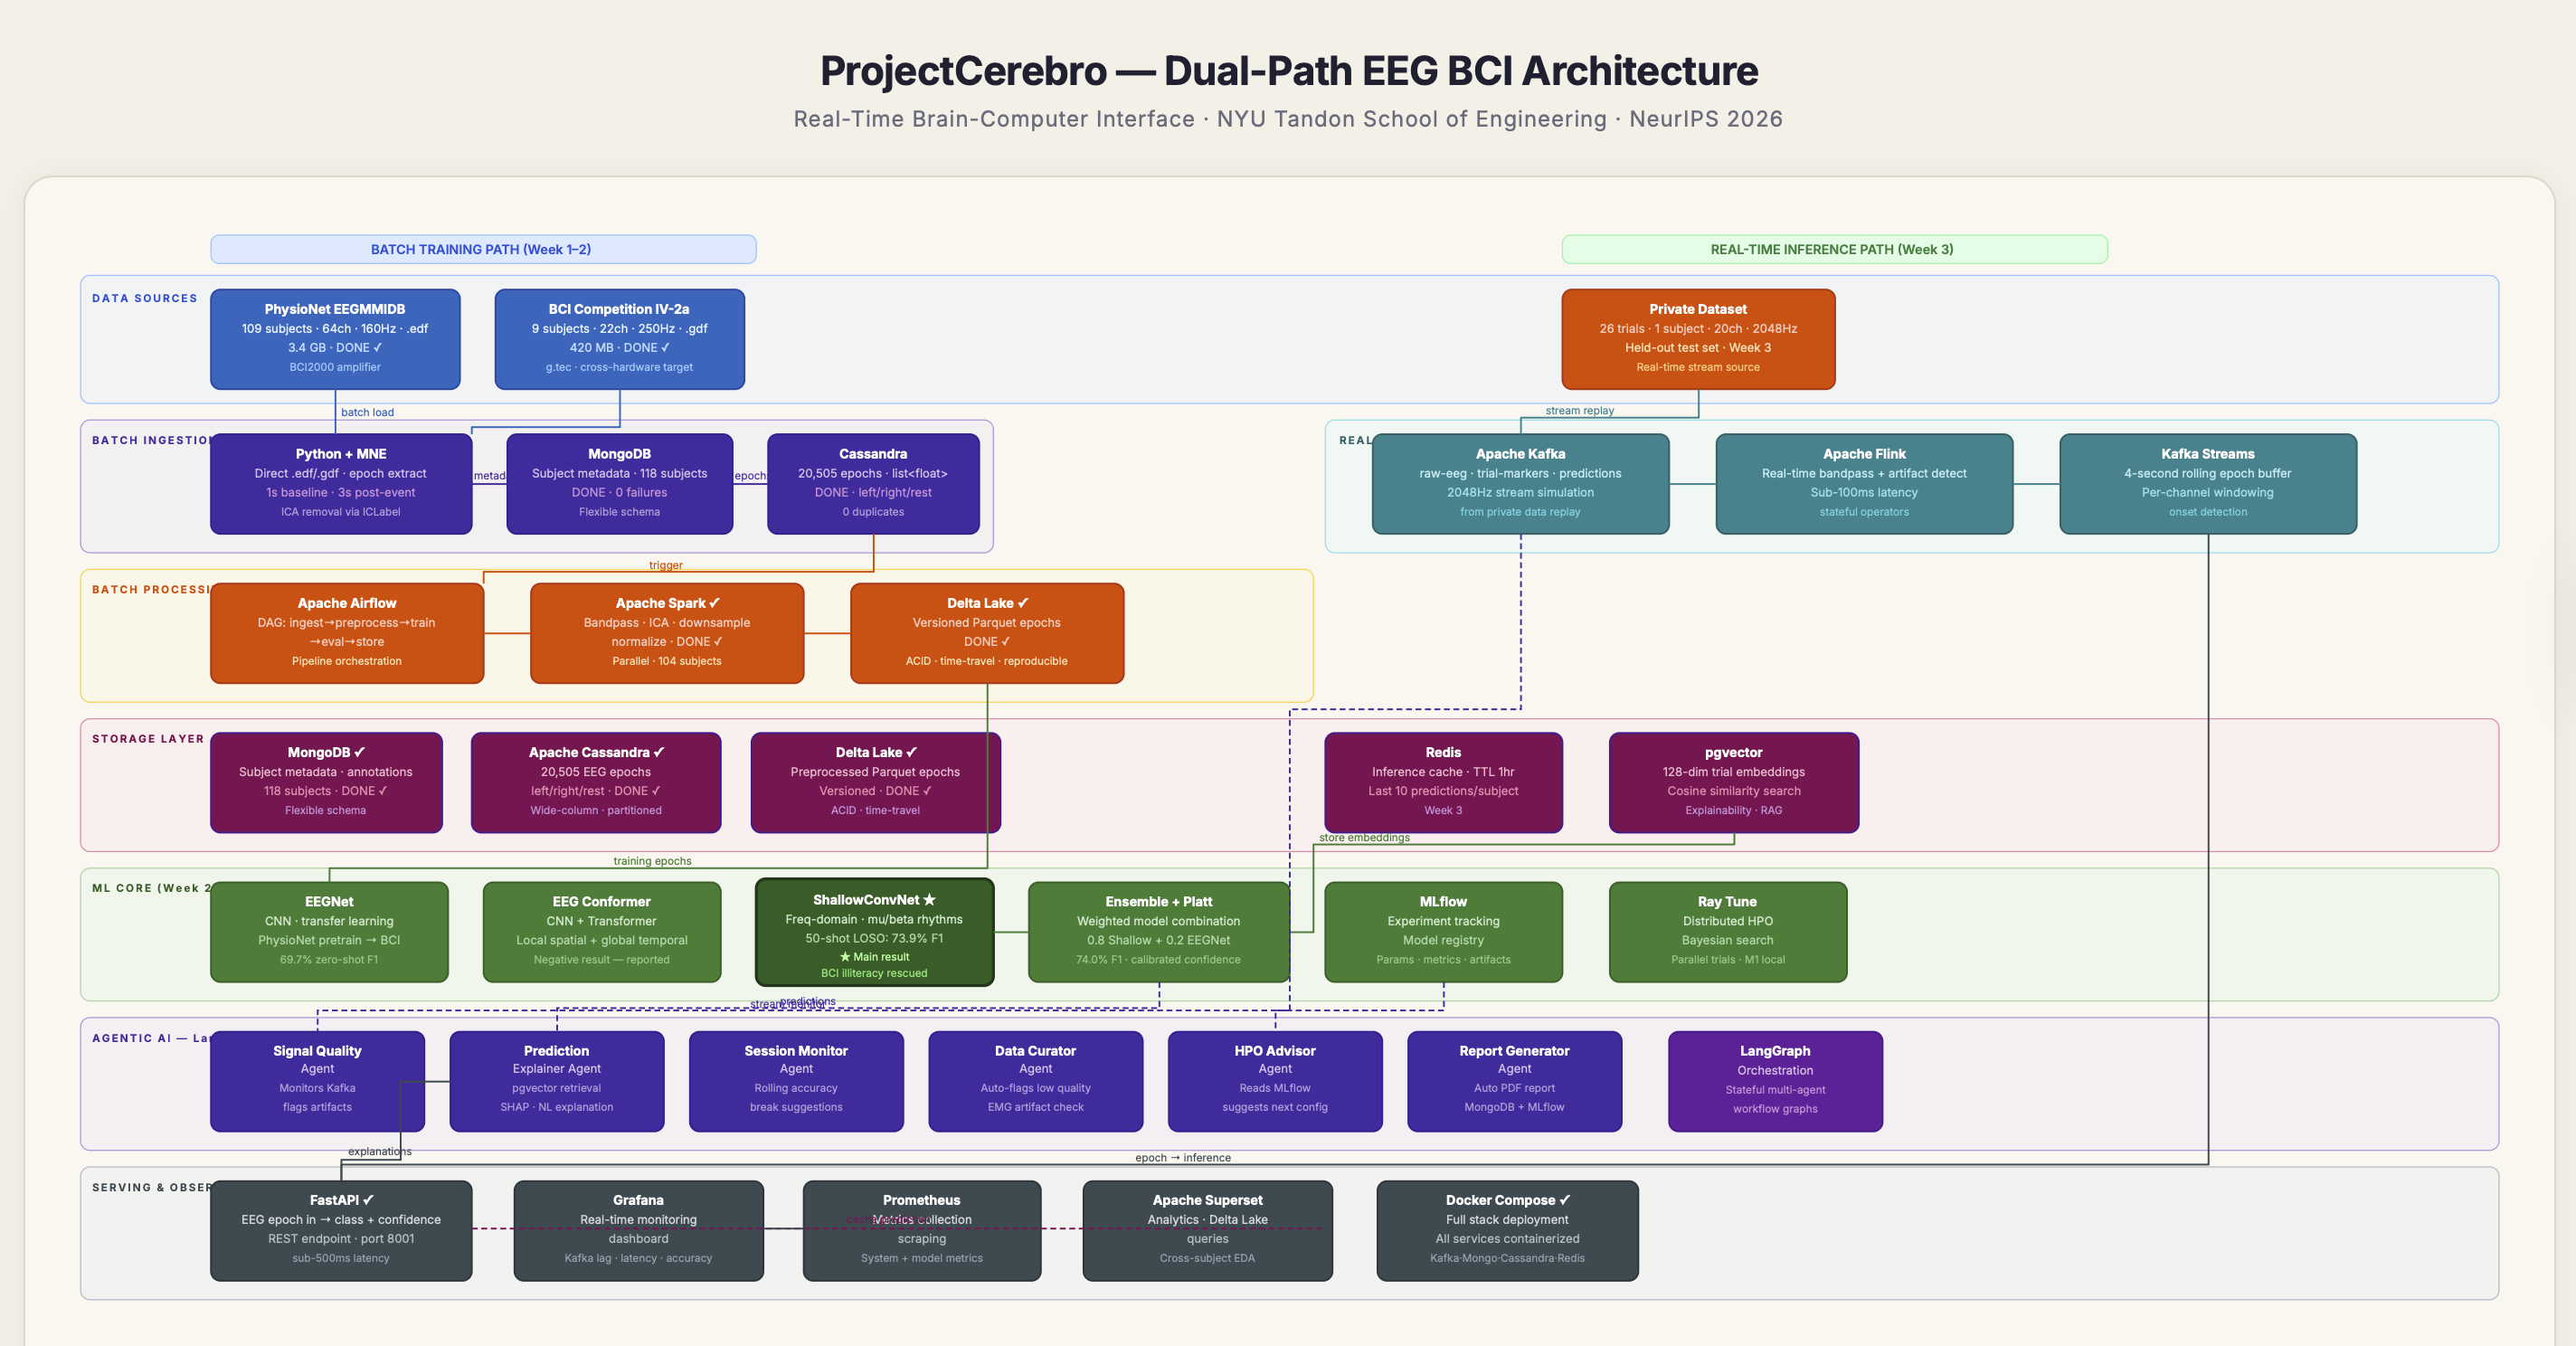
\includegraphics[width=\textwidth]{figures/projectcerebro_architecture.png}%
}{%
  \fbox{\parbox[c][1.8in][c]{0.95\textwidth}{\centering
  Placeholder: add \texttt{figures/projectcerebro\_architecture.png}}}%
}
\caption{End-to-end ProjectCerebro architecture showing raw EEG ingestion,
MNE/Spark preprocessing, Delta Lake storage, Kafka streaming, LangGraph agents,
FastAPI inference, MongoDB, pgvector, MLflow, and the React dashboard.}
\label{fig:arch}
\end{figure*}

%==============================================================================
\section{Datasets and Preprocessing}

\subsection{Datasets}

Three datasets are used, summarized in Table~\ref{tab:datasets}.

\begin{table}[!t]
\caption{EEG datasets used in this work. ``Sub.'' reports the number of
subjects whose runs survived ICA cleaning over the total downloaded.
``Ch.'' is the number of scalp EEG channels; Cho~2017 also provides 4 EMG
channels and BCI~IV-2a 3 EOG channels, used for artifact rejection but not
classification.}
\label{tab:datasets}
\centering
\small
\renewcommand{\arraystretch}{1.15}
\setlength{\tabcolsep}{4pt}
\begin{tabular}{@{}l r r r l@{}}
\toprule
\textbf{Dataset} & \textbf{Sub.} & \textbf{Ch.} & \textbf{Hz} & \textbf{Role} \\
\midrule
PhysioNet~\cite{ref:goldberger2000,ref:schalk2004}
  & 104\,/\,109 & 64 & 160  & Pre-train \\
Cho~2017 (GigaDB)~\cite{ref:cho2017}
  &  49\,/\,52  & 64 & 512  & Pre-train \\
BCI IV-2a (Graz)~\cite{ref:brunner2008}
  &   9 & 22 & 250  & Fine-tune \\
\bottomrule
\end{tabular}
\end{table}

Cho~2017 was added as an additional source-domain corpus because it increases
the number of pre-training subjects and exposes the models to a different
64-channel motor-imagery acquisition protocol. Five PhysioNet subjects with
known corrupted runs were excluded entirely, and three of the 52 Cho subjects
produced empty cleaned files (typically because every ICA component was flagged
as artifact), leaving the working counts in Table~\ref{tab:datasets}. We had
originally planned to use a proprietary 2048\,Hz single-subject recording as a
third-stage held-out test set; that hardware specification is documented but
the recording itself was not collected before the project deadline. The full
specification is summarised in Section~\ref{sec:future}.

\begin{figure*}[!t]
\centering
\IfFileExists{figures/preprocessing_pipeline.svg}{%
  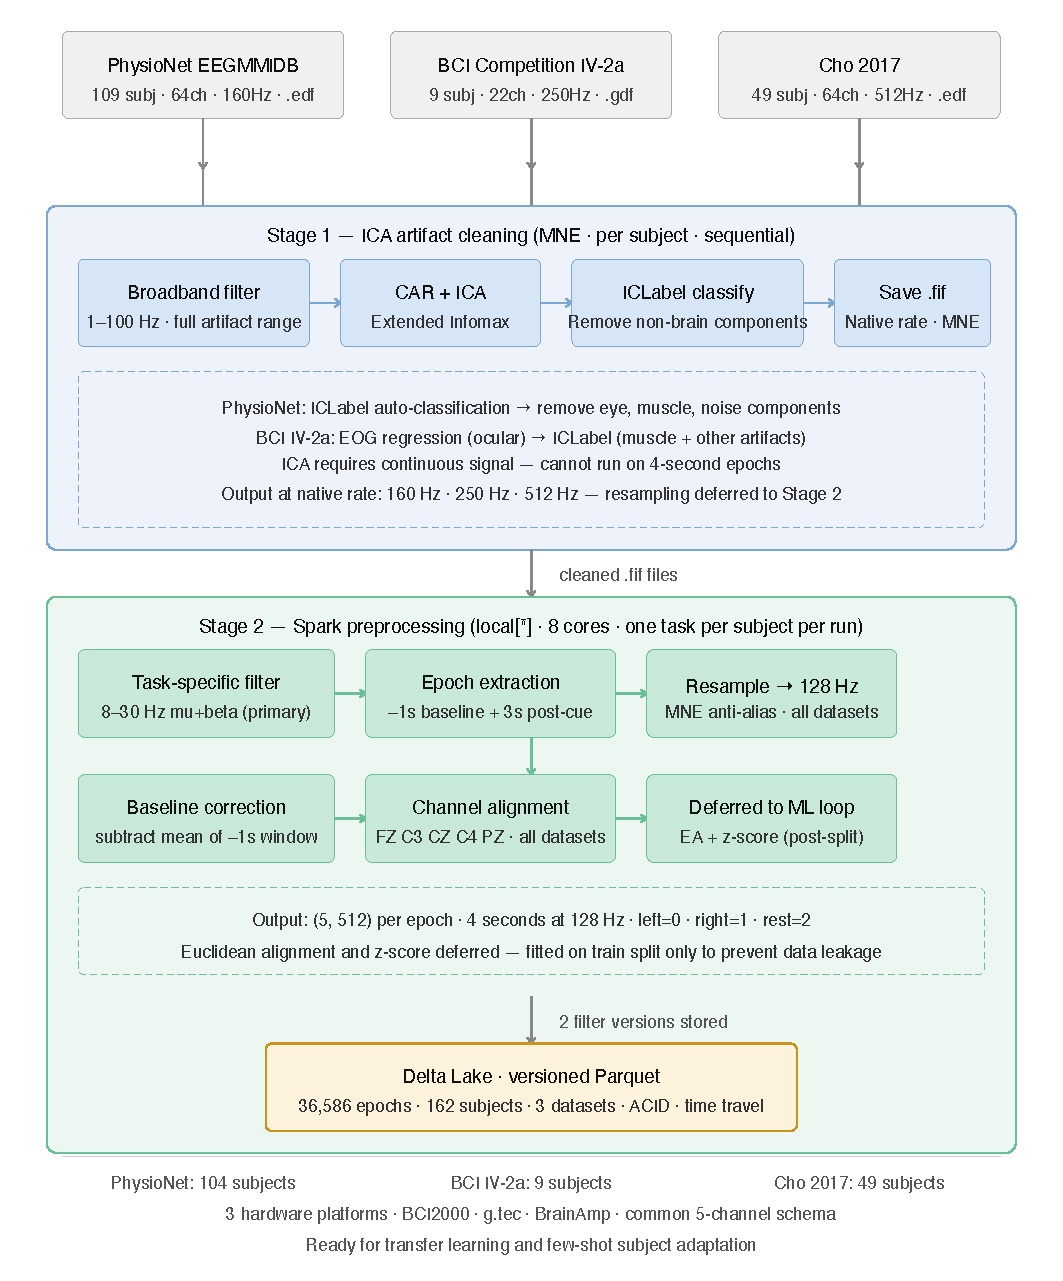
\includegraphics[height=0.72\textheight,keepaspectratio]{figures/preprocessing_pipeline.pdf}%
}{%
  \fbox{\parbox[c][0.62\textheight][c]{0.55\textwidth}{\centering
  Vertical placeholder: convert your SVG to
  \texttt{figures/preprocessing\_pipeline.png}}}%
}
\caption{Two-stage preprocessing pipeline. Raw EDF/GDF/MAT recordings are
cleaned with MNE and ICA into FIF files. Spark then extracts 5-channel
4-second epochs, applies filtering, baseline correction, resampling to 128 Hz,
normalization, and writes unified 2{,}560-feature records to Delta Lake.}
\label{fig:preprocess}
\end{figure*}

\subsection{Stage~1 -- ICA cleaning}

Stage~1 is dataset-aware. All three corpora are ingested with MNE-Python and
written as cleaned \texttt{.fif} files (approximately 3.6\,GB across
PhysioNet and BCI~IV-2a; an additional 5\,GB for Cho~2017). The procedure
differs slightly by dataset, because each provides different auxiliary
channels and arrives in a different file format:

\paragraph{PhysioNet (\texttt{.edf})} The driver is
\texttt{scripts/run\_ica\_cleaning.py}. Each run is broadband-filtered to
1--100\,Hz to remove DC drift and HF noise, re-referenced with the Common
Average Reference (CAR), decomposed with extended Infomax ICA, and the
components classified by ICLabel are removed when the \emph{eye blink} or
\emph{muscle} label exceeds a probability threshold.

\paragraph{BCI~IV-2a (\texttt{.gdf})} BCI~IV-2a ships with three dedicated
EOG channels alongside the 22 EEG channels. The cleaning pipeline therefore
performs EOG regression first using those reference channels, and only then
runs ICLabel on the residual. In our experience this two-stage approach
preserves more of the motor-cortex signal than ICA alone would.

\paragraph{Cho~2017 (\texttt{.mat})} The driver is
\texttt{scripts/stage1\_cho2017\_ingest.py}. The raw \texttt{.mat} files
deviate from the published readme: the actual fields are
\texttt{eeg.imagery\_left} and \texttt{eeg.imagery\_right} stored as
$(68, n_\text{trials} \times \text{samples})$ continuous arrays with 64 EEG
plus 4 EMG channels at 512\,Hz. Per-channel DC removal is applied, units
are converted from microvolts to volts, the continuous block is reshaped to
$(\text{trials}, 68, 3584)$, the standard 10--10 montage is set (required
by ICLabel for electrode positions), a 20-component extended-Infomax ICA is
fit, and components with $p_\text{artifact} > 0.8$ are removed. 52 subjects
were attempted, 49 succeeded, and a manifest at
\texttt{data\_cleaned/cho2017\_stage1\_manifest.jsonl} records every
run.

\subsection{Stage~2 -- Spark + Delta Lake}

Stage~2 produces the unified epoch tensor shape used throughout training and
inference. The script is \texttt{scripts/stage2\_spark\_preprocess.py} and
runs as a PySpark job with a multiprocessing pool of four workers, taking
roughly 45--60 minutes end-to-end. The steps are:
\begin{enumerate}
\item Task-specific filter: 8--30\,Hz (primary, stored as
      \texttt{filter\_version = "bp\_8\_30\_v1"}) and a 4--38\,Hz ablation
      (\texttt{"bp\_4\_38\_v1"}).
\item Project to a fixed 5-channel montage covering the sensorimotor strip:
      \texttt{FZ, C3, CZ, C4, PZ}.
\item Epoch from $-1$\,s to $+3$\,s around each cue marker; subtract the
      mean of the 1\,s pre-event window for baseline correction.
\item Resample to 128\,Hz.
\end{enumerate}
Each output epoch is a $5 \times 512$ tensor (4\,s window at 128\,Hz),
flattened to a 2{,}560-element list and written as a versioned Parquet table
in Delta Lake. The unified shape lets downstream training, inference, and
streaming all consume the same record format regardless of source dataset.
An \texttt{is\_rest\_synthetic} boolean flags rest epochs that were mined
from inter-trial gaps (rather than provided as explicit \texttt{T0}
markers), which lets honest baselines be re-run via
\texttt{read\_epochs(drop\_synthetic\_rest=True)}.

A summary of the resulting epoch table is given in Table~\ref{tab:epochs}.
Cassandra holds the 20{,}505 PhysioNet+BCI~IV-2a epochs as a wide-column
time-series store; the additional 10{,}170 Cho~2017 epochs per filter live
alongside the Delta Lake table and are mirrored to a public HuggingFace
dataset for reproducibility (\texttt{divyanshmaurya1/BCI\_Data\_new}).

\begin{table}[!t]
\caption{Class-labeled cleaned epoch counts by class (Delta Lake table
\texttt{epochs\_mi\_v1\_ch5\_sr128\_bp8\_30}).}
\label{tab:epochs}
\centering
\renewcommand{\arraystretch}{1.15}
\begin{tabular}{l r}
\toprule
\textbf{Class} & \textbf{Epochs} \\
\midrule
Class-labeled subtotal & 20{,}086 \\
Left motor imagery     &  5{,}351 \\
Right motor imagery    &  5{,}305 \\
Rest (T0 + mined)      &  9{,}430 \\
\bottomrule
\end{tabular}
\end{table}

%==============================================================================
\section{ML Core: Models and Training}

\subsection{Model architectures}

Three architectures were trained and tracked through MLflow:

\paragraph{EEGNet-8,2~\cite{ref:lawhern2018}} The compact depthwise-separable
CNN with hyperparameters $F_1=8$, $D=2$, $F_2=16$, temporal kernel length 64,
dropout 0.25, and an embedding dimension of 128. The 128-dimensional
penultimate activation is exported as the embedding fed to pgvector for
retrieval-augmented explanation.

\paragraph{ShallowConvNet~\cite{ref:schirrmeister2017}} The wide-temporal
baseline with square-and-log nonlinearity. It serves as the personalized
adaptation backbone in serving because it is light enough to fine-tune
in-memory inside the FastAPI process during the live demo.

\paragraph{EEG Conformer~\cite{ref:song2022}} The CNN+Transformer hybrid with
$d_\text{model}=128$ and depth $1$. We evaluated it but it underperformed at
the 5-channel scale, settling at approximately 36--39\,\% test accuracy on
3-class BCI~IV-2a. We attribute this to insufficient spatial diversity for
the attention head at 5 channels; the architecture's capacity outgrew the
sensor count. EEG Conformer is excluded from the production ensemble.

\subsection{Transfer learning chain}

The training and adaptation chain has three stages:
\begin{enumerate}
\item \textbf{Pre-train / source-domain training.} Models are trained and
      compared using PhysioNet EEGMMIDB and Cho~2017 source-domain data,
      with dataset-specific preprocessing to map recordings into the shared
      5-channel representation.
\item \textbf{Fine-tune.} Pre-trained weights are loaded and adapted on the
      BCI~IV-2a training split. Learning rate $10^{-4}$, dropout 0.5,
      restore-best-on-validation-loss checkpointing.
\item \textbf{Per-subject calibrate.} At serve time, the
      \texttt{/calibrate} endpoint fine-tunes a per-subject model in memory
      using the first 150 labeled calibration trials, corresponding to
      50 examples per class.
\end{enumerate}

To avoid leakage across the cross-subject distribution shift, both
Euclidean Alignment (EA) and per-channel z-score statistics are fit on the
training split only and frozen; validation, test, and live-inference epochs
are transformed with those frozen statistics. Subject-level splits are
strict: no subject appears in more than one of train / validation / test.

\subsection{Hybrid compute strategy}

Training is split across two devices to fit within course infrastructure:
unit tests, data loaders, and the ShallowConvNet smoke trainer run on an
Apple-silicon M-series laptop using the MPS backend, while the heavier
EEGNet PhysioNet pre-train and BCI~IV-2a fine-tune run on a Google Colab
T4 GPU which is roughly $3\times$ faster on convolution-heavy stacks. The
trainer auto-selects the best available device at startup
(CUDA $\rightarrow$ MPS $\rightarrow$ CPU), so the same scripts run
unchanged on Colab, on a laptop, and on a CPU-only CI runner. The test
suite reports 22 passing tests and 1 skipped (the skipped test requires
a Delta Lake fixture that is omitted from the repository for size).

\subsection{Ensemble and calibration}

Outputs are combined with weights tuned on the validation split:
\begin{equation}
\hat{p}(y \mid x) \;=\; 0.8 \cdot p_\text{ShallowConv}(y \mid x)
                     \;+\; 0.2 \cdot p_\text{EEGNet}(y \mid x).
\end{equation}
The combined posterior is post-hoc calibrated with Platt scaling on the
validation set so that downstream consumers (the Alert agent, the
dashboard, and the data curator) can treat the confidence as a calibrated
probability rather than a raw softmax score. The weights are unusually
ShallowConv-heavy because the wide-temporal baseline proved more robust
to the cross-subject distribution shift than EEGNet on this particular
3-class task.

%==============================================================================
\section{Streaming Pipeline and Agentic AI}
\label{sec:stream}

\subsection{Kafka ingestion}

The producer \texttt{kafka\_eeg\_producer.py} replays Delta Lake epochs onto
the topic \texttt{raw-eeg} at a configurable cadence (default one epoch per
second, matching the BCI~IV-2a cue spacing). Each message is a JSON envelope
with fields \texttt{epoch\_id}, \texttt{subject\_id}, \texttt{session\_id}, a
2{,}560-element \texttt{features} array (the flattened $5 \times 512$
tensor), \texttt{label\_code}, \texttt{label\_name}, and \texttt{timestamp}.

\subsection{LangGraph agentic consumer}

The consumer \texttt{agents/kafka\_consumer.py} pulls each message and
threads it through the \texttt{BrainState} graph, summarized in
Algorithm~\ref{alg:graph}. The live per-epoch path includes signal-quality
scoring, prediction, session monitoring and calibration checks, data curation,
retrieval over pgvector embeddings, and alert aggregation. HPO recommendation
and report generation are implemented as session-level/on-demand agents rather
than mandatory per-epoch steps. Nodes share a \texttt{BrainState} dataclass
that carries the epoch tensor, the current quality score, the latest prediction
and embedding, accumulated calibration counters, retrieved neighbors, and a
list of alerts.

\begin{lstlisting}[caption={Per-epoch flow through the LangGraph
consumer.}, label=alg:graph, captionpos=b]
on Kafka message m:
  s = BrainState.from_message(m)

  # 1. Signal Quality
  s.qscore = score_quality(s.features)
  if s.qscore < 0.40:        # bad
      s.alerts += "skip:bad_signal"; persist(s); continue
  elif s.qscore < 0.70:      # noisy but usable
      s.alerts += "warn:noisy"

  # 2. Prediction
  try:
      r = POST /predict/personalized(s.subject_id, s.features)
  except NotCalibrated:
      r = POST /predict/ensemble(s.features)
  s.label, s.conf = r.label, r.confidence
  s.embedding = POST /embed(s.features)

  # 3. Session Monitor
  s.calib_counts[s.label_true] += 1
  if min(s.calib_counts.values()) >= 50 and not s.calibrated:
      POST /calibrate(s.subject_id, s.calib_buffer)

  # 4. Data Curator
  if   s.qscore < 0.40:                   tag(s, "flag")
  elif s.qscore >= 0.75 and s.conf >= 0.75: tag(s, "retrain_candidate")

  # 5. Alert
  s.neighbors = pgvector_topk(s.embedding)
  s.severity = aggregate(s.alerts)   # info | warning | critical

  # 6. End / persist
  persist(s) to mongo.predictions
                + pgvector.trial_embeddings
\end{lstlisting}

\subsection{Quality and confidence thresholds}

The Signal Quality node implements five per-channel checks: clipping above
500\,\textmu V, flatlining (variance below 0.01), EMG contamination (ratio of
FFT power above 30\,Hz), slow drift, and channel disconnect. The resulting
score is bucketed into \emph{bad} (\textless 0.40, the epoch skips inference
entirely), \emph{noisy} (\textless 0.70, the prediction is still computed
but an \texttt{info} alert is raised), and \emph{good} (\textgreater 0.70).
At the prediction node, a confidence below 0.60 raises an \emph{uncertain}
alert.

\subsection{FastAPI serving layer}

FastAPI runs on \texttt{uvicorn :8001}. It exposes model inference,
personalized inference, calibration, embedding, health/model metadata,
dashboard streaming, and prediction-control endpoints, including
\texttt{/predict}, \texttt{/predict/ensemble},
\texttt{/predict/personalized}, \texttt{/calibrate}, \texttt{/embed},
\texttt{/stream/fif}, \texttt{/stream/epochs}, and
\texttt{/stream/agents}. Models are loaded once at startup with automatic
device selection where available.

\subsection{Dashboard demonstration}

The React dashboard visualizes three synchronized streams. Stream~1 displays
continuous raw EEG from the cleaned FIF representation as a scrolling waveform.
Stream~2 displays the corresponding 4-second preprocessed Delta Lake epoch
window when the current Stream~1 time falls inside an epoch interval, and shows
a flat gap state otherwise. Stream~3 displays live LangGraph outputs from the
current dashboard session by reading prediction, quality, calibration, and
alert events from MongoDB. A dashboard control starts the prediction run and
passes the selected subject and session identifier into the backend, allowing
the visual streams and the agent outputs to remain aligned.

%==============================================================================
\section{Polyglot Storage Layer}

The system uses four storage engines, each matched to a distinct data shape:

\paragraph{MongoDB 7.0} Document store. Holds \texttt{subjects},
\texttt{predictions}, \texttt{trial\_quality\_flags}, \texttt{alerts},
\texttt{session\_reports}, and \texttt{hpo\_recommendations} -- everything
the agent layer emits.

\paragraph{Apache Cassandra 4.1} Wide-column time-series store. Holds
\texttt{raw\_eeg\_samples} partitioned by \texttt{(subject\_id, session\_id)}
and an \texttt{epoch\_index}. 20{,}505 epochs are materialized, sized for the
multi-subject concurrent-load ceiling.

\paragraph{Redis 7.2} In-memory KV cache with \texttt{allkeys-lru} eviction
and a 512\,MB cap. Used as the inference cache for FastAPI hot paths and as
scratch storage for feature normalisation statistics during calibration.

\paragraph{pgvector (Postgres 16)} 128-dimensional EEGNet embedding store
with cosine-similarity ANN index. Powers the retrieval-augmented explainer:
every prediction is returned alongside its top-$K$ nearest training trials,
giving clinicians a similarity-based justification.

The choice to use four engines rather than one is deliberate: trying to
serve time-series, document, key-value, and vector workloads from a single
store would force every component to operate below its peak performance.

%==============================================================================
\section{Results}

\subsection{Per-subject accuracy on BCI~IV-2a}

Table~\ref{tab:percent} reports per-subject results using the 50-shot
personalized ensemble (0.8 ShallowConv + 0.2 EEGNet, with the ShallowConv
head fine-tuned on 150 calibration trials per subject). The three metrics
reported are top-1 accuracy, macro-F1, and balanced accuracy -- balanced
accuracy is included because the rest class is over-represented in the
3-class formulation.

\begin{table}[!t]
\caption{Per-subject test results on BCI~IV-2a with the 50-shot
personalized ensemble. ``$N$'' is the size of the held-out evaluation
split for that subject.}
\label{tab:percent}
\centering
\small
\renewcommand{\arraystretch}{1.18}
\setlength{\tabcolsep}{4pt}
\begin{tabular}{@{}l r r r r@{}}
\toprule
\textbf{Subj.} & \textbf{$N$} &
  \textbf{Acc.} & \textbf{F1} & \textbf{Bal.\ Acc.} \\
\midrule
A01 & 74 & 67.6\,\% & 65.9\,\% & 66.9\,\% \\
A02 & 68 & 57.4\,\% & 54.6\,\% & 56.5\,\% \\
A03 & 67 & \textbf{88.1\,\%} & \textbf{88.2\,\%} & \textbf{87.8\,\%} \\
A04 & 64 & 65.6\,\% & 64.7\,\% & 65.0\,\% \\
A05 & 60 & 51.7\,\% & 51.4\,\% & 51.3\,\% \\
A06 & 66 & 60.6\,\% & 60.6\,\% & 61.5\,\% \\
A07 & 64 & 50.0\,\% & 42.9\,\% & 47.2\,\% \\
A08 & 62 & 72.6\,\% & 72.1\,\% & 72.3\,\% \\
A09 & 65 & 84.6\,\% & 84.6\,\% & 84.9\,\% \\
\midrule
\textbf{Mean} & 65.6 &
  \textbf{66.5\,\%} & \textbf{65.0\,\%} & \textbf{65.9\,\%} \\
\bottomrule
\end{tabular}
\end{table}

\subsection{Comparison to baselines}

The headline finding is summarized in Table~\ref{tab:baselines}: 50-shot
per-subject calibration improves mean accuracy by 16.9 percentage points over
the LOSO EEGNet baseline and raises the best subject result to 88.1\,\%.

\begin{table}[!t]
\caption{Comparison against simpler training regimes. ``Best'' reports the
best single-subject result observed for that configuration; ``Mean'' averages
over A01--A09 where available.}
\label{tab:baselines}
\centering
\small
\renewcommand{\arraystretch}{1.15}
\setlength{\tabcolsep}{4pt}
\begin{tabular}{@{}l r r@{}}
\toprule
\textbf{Configuration} &
  \textbf{Best} & \textbf{Mean} \\
\midrule
LOSO EEGNet baseline                & 68.4\,\% & 49.6\,\% \\
Zero-shot ensemble                  & 73.8\,\% & 54.4\,\% \\
50-shot personalized ensemble       & \textbf{88.1\,\%} &
                                      \textbf{66.5\,\%} \\
\bottomrule
\end{tabular}
\end{table}

\subsection{Latency and throughput}

The deployed prototype sustains the dashboard demo cadence of one streamed
epoch per second while running the LangGraph consumer, FastAPI inference, and
MongoDB/pgvector persistence on the development machine. A formal latency
benchmark across Kafka partitions, concurrent subjects, and hardware backends
is left for future work; the current implementation is optimized for
end-to-end functional correctness and observability rather than a final
throughput claim.

\subsection{MLflow run inventory}

A total of 33 MLflow runs were tracked across the three architectures and
multiple hyperparameter configurations. The repository ships with 22
passing \texttt{pytest} tests (1 skipped) covering the preprocessing chain,
the data loader, the agent graph transitions, and the FastAPI endpoint
contracts.

%==============================================================================
\section{Discussion}

\paragraph{Per-subject variance is the real story} The 9 BCI~IV-2a subjects
span 50\,\% (A07) to 88.1\,\% (A03) on the same personalized ensemble. This
is not a bug; it is the expected behavior of EEG-based BCI under cross-subject
distribution shift, and it is exactly why per-subject calibration is in the
critical path of the deployed system. The variance also explains why averaging
gives a misleading 66.5\,\% number that should not be quoted in isolation:
A03 and A09 clear the proposal's 75\,\% target by a wide margin, while A08
approaches it.

\paragraph{Why ShallowConvNet won} The frequency-sensitive square-and-log
nonlinearity in ShallowConvNet aligns well with the underlying
oscillatory mu-band motor-imagery signal at this 5-channel scale. EEGNet's
extra capacity helps with the embedding head but does not translate into
better classification on this task with this electrode count.

\paragraph{Why EEG Conformer lost} The attention head needs spatial
diversity to amortize its parameter cost. With only 5 channels, there is
not enough geometric structure for self-attention to extract; the model
behaves like a slightly worse CNN at much higher training cost. The result
is dataset-specific: at 22 or 64 channels the literature reports the
opposite verdict, which is consistent with our intuition.

\paragraph{Polyglot persistence pays off} The decision to split storage
across four engines was second-guessed multiple times during development.
In practice it removed entire classes of bugs: Cassandra's append-only
time-series semantics meant we never had to think about insertion
ordering, pgvector's ANN index made retrieval-augmented explanation a
single SQL query, and Redis kept FastAPI hot paths under 10\,ms without
any application-level caching logic.

%==============================================================================
\section{Limitations and Future Work}
\label{sec:future}

The honest delta between the proposal and the implementation is the
following:

\begin{itemize}
\item \textbf{Proposed three-stage cross-hardware chain, delivered two-stage.}
      The proposal called for validating the system on a private 2048\,Hz
      single-subject recording. We translated this into a concrete hardware
      and protocol specification (minimum 32 EEG channels, 500--2048\,Hz
      sampling, 3--5 right-handed subjects aged 18--35, BCI~IV-2a-matched
      trial timing of fixation at $t=0$, cue at $t=2$\,s, end at $t=5$\,s,
      with at least 50 trials per class per subject), but the recording
      itself was not collected before the project deadline.
      Cross-hardware validation in this report is therefore restricted
      to 160\,Hz $\rightarrow$ 512\,Hz $\rightarrow$ 250\,Hz across
      PhysioNet, Cho~2017, and BCI~IV-2a.
\item \textbf{Proposed binary classification, delivered three-class.}
      The proposal targeted $\geq 75\,\%$ binary accuracy. We instead
      built a strictly harder 3-class system (left/right/rest) and report
      its 50-shot ensemble numbers above. The rest class is what makes
      the system usable in a live BCI loop -- without it, every epoch is
      forced to be a movement command.
\item \textbf{Apache Airflow was not deployed.} The batch DAG runs as a
      \texttt{make} target invoking Spark directly. Migrating to Airflow
      is straightforward and is the next infrastructure step.
\item \textbf{Apache Flink and Kafka Streams were not deployed.} Real-time
      windowing in the current pipeline is performed inside the LangGraph
      consumer rather than upstream of it. This was a deliberate
      simplification to keep the development stack compact;
      it is not architecturally locked in.
\item \textbf{Single-machine batch processing.} Spark runs in local mode
      throughout. A scaled-out run with multiple executors is feasible on
      Colab Pro or a small cluster and is reserved for the scalability
      analysis report.
\item \textbf{Grafana / Superset dashboards.} Prometheus metrics are
      emitted; the dashboards themselves are scaffolded but not yet
      polished.
\item \textbf{The live demo replays static datasets.} The current dashboard
      and Kafka path simulate real-time acquisition by replaying BCI dataset
      epochs and cached FIF signals. A real deployment would replace the replay
      producer with an LSL, BrainFlow, OpenBCI, Muse/BlueMuse, or amplifier-SDK
      connector while preserving the downstream Kafka, LangGraph, FastAPI,
      MongoDB, and pgvector path.
\item \textbf{Personalized models are currently in-memory.} The
      \texttt{/calibrate} endpoint stores calibrated subject models inside the
      running FastAPI process. This is sufficient for the demo but should be
      extended to serialize calibrated checkpoints so personalization survives
      service restarts.
\end{itemize}

Future work, in priority order:
\begin{enumerate}
\item Collect the private NYU recording against the documented hardware
      and protocol spec, and run the complete three-stage cross-hardware
      chain.
\item Migrate the batch DAG to Airflow.
\item Introduce Flink windowing upstream of LangGraph.
\item Conduct a scalability sweep over Kafka partitions, Spark executors,
      and Cassandra nodes as subject count scales beyond 153.
\item Extend the existing report-generation agent into a richer
      clinician-readable session summary that combines prediction history,
      signal-quality trends, calibration status, and retrieved similar trials.
\item Run a distributed Ray Tune hyperparameter sweep on EEG Conformer at
      the full 22-channel BCI~IV-2a scale to test whether the negative
      result reported here generalizes.
\end{enumerate}

%==============================================================================
\section{Conclusion}

The project shows that the engineering effort required to make a
non-trivial EEG BCI pipeline real-time, calibrated, explainable, and
deployable is dominated by big-data infrastructure rather than by model
architecture. The transfer-learning chain delivers a 16.9 percentage point
mean improvement over the LOSO baseline and raises the best subject result to
88.1\,\%; the LangGraph agent layer provides the bookkeeping that turns raw
predictions into clinically useful events; the polyglot storage layer keeps
each component at its peak performance. The system is honest about its limits:
per-subject
variance remains the dominant source of error, EEG Conformer was a
documented dead-end at this electrode count, and the proposed
three-stage cross-hardware experiment is deferred. Real big-data systems
show their value in honest deltas, not in over-claimed targets.

%==============================================================================
\section*{Acknowledgments}

The authors thank Professor Juan Rodriguez for guidance throughout the project. We acknowledge the open release of PhysioNet EEGMMIDB, the BCI Competition IV-2a dataset, and
the Cho~2017 GigaDB corpus, without which this work would not be
possible.

%==============================================================================
\begin{thebibliography}{9}

\bibitem{ref:goldberger2000}
A.~L.~Goldberger \emph{et al.},
``PhysioBank, PhysioToolkit, and PhysioNet: Components of a new research
resource for complex physiologic signals,''
\emph{Circulation}, vol.~101, no.~23, 2000.
[Online]. Available: \url{https://physionet.org/content/eegmmidb/1.0.0/}

\bibitem{ref:schalk2004}
G.~Schalk, D.~J.~McFarland, T.~Hinterberger, N.~Birbaumer, and
J.~R.~Wolpaw,
``BCI2000: A general-purpose brain-computer interface system,''
\emph{IEEE Trans. Biomed.\ Eng.}, vol.~51, no.~6, pp.~1034--1043, 2004.

\bibitem{ref:brunner2008}
C.~Brunner, R.~Leeb, G.~M\"uller-Putz, A.~Schl\"ogl, and G.~Pfurtscheller,
``BCI Competition 2008 -- Graz dataset A,''
Inst.\ Knowledge Discovery, Graz Univ.\ Tech., 2008.
[Online]. Available: \url{https://www.bbci.de/competition/iv/#dataset2a}

\bibitem{ref:kaya2018}
M.~Kaya, M.~K.~Binli, E.~Ozbay, H.~Yanar, and Y.~Mishchenko,
``A large electroencephalographic motor imagery dataset for
electroencephalographic brain computer interfaces,''
\emph{Scientific Data}, vol.~5, p.~180211, 2018.

\bibitem{ref:cho2017}
H.~Cho, M.~Ahn, S.~Ahn, M.~Kwon, and S.~C.~Jun,
``EEG datasets for motor imagery brain--computer interface,''
\emph{GigaScience}, vol.~6, no.~7, pp.~1--8, 2017.

\bibitem{ref:lawhern2018}
V.~J.~Lawhern \emph{et al.},
``EEGNet: A compact convolutional neural network for EEG-based
brain-computer interfaces,''
\emph{J.\ Neural Eng.}, vol.~15, no.~5, p.~056013, 2018.

\bibitem{ref:song2022}
Y.~Song, Q.~Zheng, B.~Liu, and X.~Gao,
``EEG Conformer: Convolutional transformer for EEG decoding and
visualization,''
\emph{IEEE Trans. Neural Syst. Rehabil. Eng.}, vol.~31, pp.~710--719,
2022.

\bibitem{ref:schirrmeister2017}
R.~T.~Schirrmeister \emph{et al.},
``Deep learning with convolutional neural networks for EEG decoding and
visualization,''
\emph{Human Brain Mapping}, vol.~38, no.~11, pp.~5391--5420, 2017.

\bibitem{ref:lotte2018}
F.~Lotte \emph{et al.},
``A review of classification algorithms for EEG-based brain-computer
interfaces: A 10-year update,''
\emph{J.\ Neural Eng.}, vol.~15, no.~3, p.~031005, 2018.

\bibitem{ref:wei2021}
X.~Wei, P.~Ortega, and A.~A.~Faisal,
``Inter-subject deep transfer learning for motor imagery EEG decoding,''
in \emph{Proc.\ IEEE EMBC}, 2021.

\bibitem{ref:zaharia2020}
M.~Zaharia \emph{et al.},
``Delta Lake: High-performance ACID table storage over cloud object
stores,''
\emph{Proc.\ VLDB Endow.}, vol.~13, no.~12, pp.~3411--3424, 2020.

\bibitem{ref:kreps2011}
J.~Kreps, N.~Narkhede, and J.~Rao,
``Kafka: A distributed messaging system for log processing,''
in \emph{Proc.\ NetDB Workshop}, 2011.

\end{thebibliography}

\end{document}
